\documentclass[a4j, twocolumn]{ltjsarticle}
\usepackage{graphicx}
\usepackage{luatexja}
%\usepackage[margin=1in]{geometry} % 余白を1インチに設定
\usepackage{listings,url} %日本語のコメントアウトをする場合jvlisting(もしくはjlisting)が必要
%ここからソースコードの表示に関する設定
\usepackage{color}
\usepackage[hidelinks]{hyperref}


\definecolor{OliveGreen}{rgb}{0.0,0.6,0.0}
\definecolor{Orenge}{rgb}{0.89,0.55,0}
\definecolor{SkyBlue}{rgb}{0.28, 0.28, 0.95}
\lstset{
  basicstyle={\ttfamily},
  identifierstyle={\small},
  commentstyle={\smallitshape},
  keywordstyle={\small\bfseries},
  ndkeywordstyle={\small},
  stringstyle={\small\ttfamily},
  frame={tb},
  breaklines=true,
  columns=[l]{fullflexible},
  numbers=left,
  xrightmargin=0em,
  xleftmargin=3em,
  numberstyle={\scriptsize},
  stepnumber=1,
  numbersep=1em,
	tabsize=2,
  lineskip=-0.5ex,
  keywordstyle={\color{SkyBlue}},     %キーワード(int, ifなど)の書体指定
  commentstyle={\color{OliveGreen}},  %注釈の書体
  stringstyle=\color{Orenge}          %文字列
}

\renewcommand{\lstlistingname}{ソースコード}
\renewcommand{\labelenumi}{(\arabic{enumi})}

\begin{document}
  \section{目的}
  本レポートの目的は、シェルの内部の動作原理を理解することである。シェルとは、ユーザが入力したコマンドを解釈し、
  コマンドに応じて必要な処理を行うプログラムである。このシェルの機能を理解するために、代表的なシェルの機能である
  リダイレクトやパイプを実装することで、シェルの動作原理に関して理解を深めることを目的とする。また、他人が作成した
  洗練されたコードを読むことで、プログラムの作成方法やコードの見やすさについて学ぶことも目的とする。

  \section{設計}
    今回のシェルはパイプ、リダイレクトの実装を主としている。そのため、プログラムの流れは以下のように設計した。
    \begin{enumerate}
      \item ユーザが入力したコマンドを分割する
      \item 入力されたコマンドをすべて見る
      \item コマンドのみの時は、通常のコマンドを実行する
      \item リダイレクトがあるときは、リダイレクトを実行する
      \item パイプとリダイレクト両方があるときは、両方に対応するように処理をする。
    \end{enumerate}
  
  \section{実装}
    実装したプログラムは長いためすべては付録に記載する。ここでは、cdコマンドの処理と
    パイプとリダイレクトの処理を行っている関数について説明する。
    \subsection{cdコマンドの処理}
      次に示すコードがcdコマンドの処理を行っている関数である。
      \begin{lstlisting}[language=C,caption=cdコマンドの処理]
void cd(char **argv){
	char path[BUFSIZE];
	getcwd(path,BUFSIZE);
	if(strstr(argv[1],"/")==NULL){
		strcat(path,"/");
		strcat(path,argv[1]);
	}
	if(chdir(path)==-1){
		printf("no file\n");
		exit(1);
	}
}
      \end{lstlisting}
      引数として、標準入力で受け取った文字列を渡す。cdの後ろは相対パスが入力されると考え
      絶対パス表示にするため,getcwdを利用している。ユーザの入力の先頭に/がないと絶対パスの
      指定がうまくいかないため、/がない場合は/を追加して絶対パスを指定できるようにしている。

      \subsection{パイプリダイレクト処理}
      パイプリダイレクト処理は関数が長いため、付録で記載する。
      \begin{enumerate}
        \item 入力された文字列をすべて確認し、リダイレクトパイプの場所を記録する
        \item 通常のコマンドの場合はそのままコマンドを実行する
        \item 逆のリダイレクトがあるときは、逆のリダイレクトを実行する
        \item リダイレクトがあるときは、リダイレクトを実行する
        \item パイプとリダイレクト両方があるときは、両方に対応するように処理をする。そうでない場合は
        パイプのみを実行する。
      \end{enumerate}

  \section{リファクタリング}
    自分が作成したプログラムは、拡張性がなく、可読性が低い。コマンドとしてほかにも考えられる
    入力が存在するが、あらゆる場合に対応するとなるとプログラムがより複雑になる。そのため、
    他人が作成したプログラムを読み、コードの見やすさや拡張性について理解を得た。
    参考プログラムから、リファクタリングを施した点は次の3つである。
    \begin{enumerate}
      \item コマンドの内容を構造体で管理
      \item リスト構造でデータを柔軟に管理
      \item 逐次処理に変更
    \end{enumerate}
    次に、リファクタリングを施した3つの点を具体的に説明する。
    \subsection{コマンドの内容を構造体で管理}
      構造体は、同じ種類のデータを管理することに長けている。
      リダイレクト、パイプなどのコマンドを実行するには、必要な
      情報が異なるが、リダイレクトの処理は同じ情報で処理できる。
      このように、同じタイプのデータをまとめて構造体で管理することで、
      処理の見通しが良くなると考える。次に実際に用いた構造体の定義を示す。
      \begin{lstlisting}[language=C,caption=利用した構造体]
struct cmd{    ・・・(1)
  int type;
};

struct execcmd {     ・・・(2)
  int type;
  char *argv[MAXARGS];
};

struct redircmd {     ・・・(3)
  int type;
  struct cmd *cmd;
  char *file;
  int mode;
  int fd;
};

struct pipecmd {      ・・・(4)
  int type;
  struct cmd *left;
  struct cmd *right;
};
      \end{lstlisting}
      \begin{enumerate}
        \item 基底構造体
        \\ \indent 基底構造体の役割は、クラスの抽象化と似ている。プログラム全体を通して
        同一の型を持つ構造体を用いることで、様々な処理を統一的に管理することができる。
        \item コマンド実行構造体
        \\ \indent コマンド実行構造体は、lsやecho helloのようなコマンドを実行するための
        構造体である。argvの配列にコマンドの文字列を代入して、execvp関数で実行する。
        \item  リダイレクト構造体
        \\ \indent リダイレクト構造体は、コマンドの出力先を標準に入力からファイルに
        変更するための情報を管理するための構造体である。ここで、struct cmd *cmdは、
        出力先をファイルに変更されたコマンドである。
        \item  パイプ構造体
        \\ \indent パイプ構造体は、パイプ処理を行う部分に関する構造体である。パイプ構造体自体は
        パイプのための処理を行わず、再帰処理を行うために利用される。
      \end{enumerate}

      \subsection{リスト構造でデータを柔軟に管理}
      リスト構造は、プログラム中にデータの個数が変化するものを扱うときに
      有効である。また、リスト構造を用いると再帰処理を記述しやすい。
      例えば、リダイレクトの処理はファイルの出力先を変更することと、
      コマンド実行する2つ行う必要がある。リストでそれぞれの手順を示すことができれば
      簡潔にコードを記述できる。
      次に示すコードはリダイレクト部分を記述したruncmdを
      一部抜粋したものである。

      \begin{lstlisting}[language=C,caption=runcmd一部抜粋]
case REDIR:
  rcmd = (struct redircmd*)cmd;・・・(1)
  int fd=open(rcmd->file, rcmd->mode, S_IRUSR | S_IWUSR | S_IRGRP | S_IROTH);
  if (fd < 0) {
    perror("open failed");
    exit(-1);
  }
  dup2(fd,rcmd->fd);
  close(fd);
  runcmd(rcmd->cmd);  ・・・(2)
  break;
      \end{lstlisting}
      \begin{enumerate}
        \item キャスト
        \\ \indent 基底構造体であるcmdを、特定の構造体にキャストすることでリダイレクト構造体に
        変更することができる。リダイレクト構造体にキャストされたものは、リダイレクト情報をメンバに持つ。
        \item 再帰処理
        \\ \indent この再帰処理は、リダイレクト構造体のメンバであるcmdを引数としてもう一度runcmdを
        行う。これにより、出力先を変更した後にコマンドを実行することができる
      \end{enumerate}

      \subsection{逐次処理に変更}
      自分が作成したプログラムは、コマンド一度すべて見てからどのようなコマンドが入力を
      されたか確認し、コマンドに応じた処理を行う。それに対して、修正したプログラムは先頭から
      文字列を見ていき、リダイレクトやパイプの場合はどうすればいいかを同一の手順で行うようにする。
      次に示すコードはparsecmdの一部を抜粋したコードである。
      \begin{lstlisting}[language=C,caption=parsecmd一部抜粋]
exe = execcmd();
cmd = (struct execcmd*)exe;
while(argv[idx]!=NULL){
  if(strchr("<>",argv[idx][0])){
    if(strchr("<>|",argv[idx+1][0])){    ・・・(1)
      printf("syntax error\n");
      exit(-1);
    }
    switch(argv[idx][0]){    ・・・(2)
      case '<':
        exe=redircmd(exe,argv[idx+1],O_RDONLY, 0);
        break;
      case '>':
        if(argv[idx][1]=='>'){
          exe=redircmd(exe,argv[idx+1],O_WRONLY|O_CREAT, 1);
        }else{
          exe=redircmd(exe,argv[idx+1],O_WRONLY|O_CREAT, 1);
        }
        break;
    }
    
    idx+=2;
  }else if(strcmp(argv[idx],"|")==0){
    idx++;
    exe=pipecmd(exe,parsepipe(argv));    ・・・(3)
  } else { // コマンドのとき
    argc=0;
    while(argv[idx]!=NULL){              ・・・(4)
      if(strchr("<>",argv[idx][0])){
        break;
      }else if(strcmp(argv[idx],"|")==0){
        break;
      }else{
        cmd->argv[argc++]=argv[idx];
        idx++;
      }
    }
    cmd->argv[argc]=NULL;
  }
}
idx=0;
return exe;
      \end{lstlisting}
      \begin{enumerate}
        \item エラー処理
        \\ \indent リダイレクトの記号の次のコマンドブロックに、また同じリダイレクトまたはパイプ記号が存在するとき、
        コマンド書き方がおかしいとして、syntax errorと出力するようにした。
        \item リダイレクトの種類を検出
        \\ \indent リダイレクトの記号の種類を判別して、記号に応じて処理を変更する。
        \item パイプの再帰処理
        \\ \indent パイプの左のポインタには、パイプのひとつ前のコマンドの構造体のアドレスを格納する。
        右には、パイプの後のコマンド内容を書き込む
        \item コマンド処理
        \\ \indent コマンドを見つけた場合は、リダイレクトやパイプの記号になるまでcmd構造体のargvに
        コマンド文字列を代入する。
      \end{enumerate}

      \section{実験}
      今回の実験は、リファクタリングしたコードは本来通りの動きを実現できていることとともに、
      コマンドが間違っている場合は正常にコマンド実行されず、syntax errorと出力されるか確認する。
      次に、シェルプログラムを実行したときの実行結果である。
      \begin{figure}[h]
        \centering
        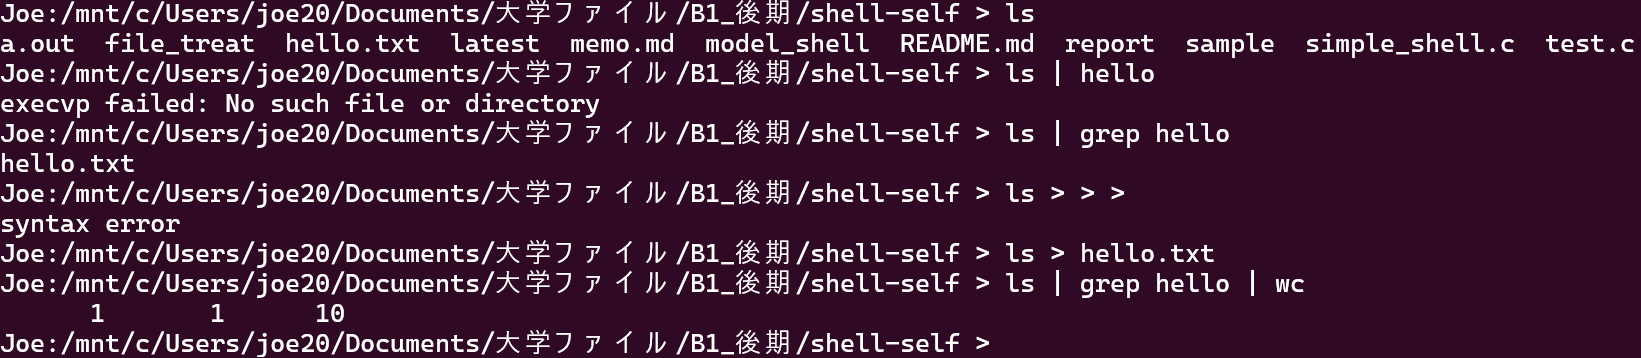
\includegraphics[width=0.4\textwidth]{image/シェル実行結果.png} % ファイル名を指定
        \caption{自作シェル実行結果}
        \label{fig:自作シェル実行結果}
      \end{figure}
      ls > >と入力した場合はシェル上にsyntax errorと表示され、コマンドの書き方が間違っていると
      指摘している。通常のコマンド、パイプの実行、パイプが多段になった場合でも正常にプログラムが
      動作していることがわかる。また、リダイレクトの処理が正しく行われていることを確認するために、
      hello.txtの内容を次に示す。
      
      \begin{figure}[h]
        \centering
        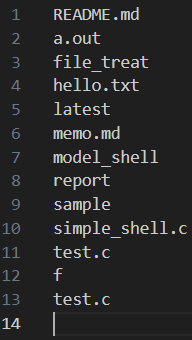
\includegraphics[width=0.2\textwidth]{image/ls実行結果.png} % ファイル名を指定
        \caption{hello.txt中身}
        \label{fig:hello.txt中身}
      \end{figure}
      確かに、lsの出力内容がhello.txtに反映されていることがわかる。

      \section{まとめ}
      本レポートでは、シェルの動作原理とリファクタリングについて学ぶことを目的とした。
      空白で区切られたコマンドの形式が定まっていることで、コマンドを容易に処理することが
      できるのだと理解した。また、リファクタリングを行ったことで、リスト構造をうまく利用して
      簡潔かつ拡張性に優れたコードを記述する技術を取得できた。


  \renewcommand{\thelstlisting}{\arabic{lstlisting}}  % リスト番号を付録ごとに1から始める
  \setcounter{lstlisting}{0}  % リストの番号を付録セクションごとに1から始める
      \newpage
  \section*{付録}
  \renewcommand{\lstlistingname}{付録}
  \begin{lstlisting}[language=C,caption=パイプリダイレクト関数]
void PipeRedirect(char **argv){
  int is_redirect=0;
  int is_oppose_redirect=0;
  int *pipe_locate=NULL;
  pipe_locate=(int*)malloc(sizeof(int));
  pipe_locate[0]=-1;
  int pipe_count=0;
  
  for(int i=0;argv[i]!=NULL;i++){     ・・・(1)
    if(strcmp(argv[i],">")==0){
      is_redirect=i;
      argv[i]=NULL;
    }else if(strcmp(argv[i],"<")==0){
      is_oppose_redirect=i;
      argv[i]=NULL;
    }else if(strcmp(argv[i],"|")==0){
      pipe_count++;
      pipe_locate=realloc(pipe_locate,(pipe_count+1) * sizeof(int));
      pipe_locate[pipe_count]=i;
      argv[i]=NULL;
    }
  }

  int pipefd[pipe_count+1][2];

  if(pipe_count==0 && is_redirect==0 && is_oppose_redirect==0){   ・・・(2)
    if(fork()==0){
      if(execvp(argv[0],argv)){           
        perror("execvp");
        exit(EXIT_FAILURE);
      }		
    }
  }else if(is_oppose_redirect!=0){            ・・・(3)
    if(fork()==0){
      if(is_FileOrDir(argv[is_redirect+1])==0){
        exit(1);
      }
      if(is_FileOrDir(argv[is_oppose_redirect+1])==0){
        exit(1);
      }
      int fd_in=open(argv[is_oppose_redirect+1],O_RDONLY);
      dup2(fd_in,STDIN_FILENO);
      close(fd_in);
      if(is_redirect!=0){
        int fd_out=open(argv[is_redirect+1], O_CREAT | O_WRONLY, S_IRUSR | S_IWUSR | S_IRGRP | S_IROTH);
        dup2(fd_out,STDOUT_FILENO);
        close(fd_out);
      }
      if(execvp(argv[0],argv)){
        perror("execvp");
        exit(EXIT_FAILURE);
      }
    }
  }else if(is_redirect!=0 && pipe_count==0){       ・・・(4)
    if(fork()==0){
      if(is_FileOrDir(argv[is_redirect+1])==0){
        exit(1);
      }
      int fd=open(argv[is_redirect+1], O_CREAT | O_WRONLY, S_IRUSR | S_IWUSR | S_IRGRP | S_IROTH);
      dup2(fd, 1);
      close(fd);
      if(execvp(argv[0],argv)){
        perror("execvp");
        exit(EXIT_FAILURE);
      }
    }
  }else{     ・・・(5)
    for(int i=0;i<pipe_count+1;i++){
      if(i!=pipe_count){
        pipe(pipefd[i]);
      }
      if(fork()==0){
        if(i==0){
          close(pipefd[i][0]);
          dup2(pipefd[i][1],STDOUT_FILENO);
          close(pipefd[i][1]);
        }else if(i==pipe_count){
          dup2(pipefd[i-1][0],STDIN_FILENO);
          close(pipefd[i-1][0]);
          if(is_redirect){
            int fd=open(argv[is_redirect+1], O_CREAT | O_WRONLY, S_IRUSR | S_IWUSR | S_IRGRP | S_IROTH);
            dup2(fd, 1);
            close(fd);
          }
          close(pipefd[i-1][1]);
        }else{
          close(pipefd[i][0]);
          close(pipefd[i-1][1]);
          dup2(pipefd[i-1][0], STDIN_FILENO);
          dup2(pipefd[i][1], STDOUT_FILENO);
          close(pipefd[i][1]);
          close(pipefd[i-1][0]);
        }
        if(execvp(argv[pipe_locate[i] + 1], argv + pipe_locate[i] + 1) < 0){
          perror("execvp");
          exit(EXIT_FAILURE);
        }
      }else{
      }
    }
  }
  for(int i=0;i<pipe_count-1;i++){
    wait(NULL);
  }
  free(pipe_locate);
}
  \end{lstlisting}


  
  \begin{thebibliography}{99}
		\bibitem{knuth1984}
			エラトステネスのふるい,
			2024/12/15,
			\url{https://algo-method.com/descriptions/64}

    \bibitem{knuth1984}
			webpia,
			2024/12/15,
			\url{https://webpia.jp/quick_sort/}

      \bibitem{knuth1984}
			Qiita,
			2024/12/15,
			\url{https://qiita.com/cotrpepe/items/1f4c38cc9d3e3a5f5e9c}
			
	\end{thebibliography}


\end{document}